% ══════════════════════════════════════════════════════════════════
%  HR MASTERPACK — 10 pages. Warm. Human. Story-driven.
%  Reading this should feel like MEETING the candidate.
%  Compile AFTER the gallery (it embeds g2, g9, g12, g16 PDFs).
%  Compile: xelatex hr-masterpack.tex   (from this directory)
% ══════════════════════════════════════════════════════════════════
\documentclass[10pt]{article}
\usepackage[a4paper, margin=1.8cm, bottom=2.2cm]{geometry}
% ══════════════════════════════════════════════════════════════════
%  MASTERPACK SHARED PREAMBLE
%  Every document in this package inputs this ONE file (relative path),
%  then palette / identity / typography / components / backgrounds.
%  Engine: XeLaTeX. Compile from the file's own directory.
% ══════════════════════════════════════════════════════════════════
\usepackage{tikz}
\usetikzlibrary{
  arrows.meta, shapes.geometric, shapes.symbols, shapes.misc,
  positioning, shadows.blur, shadows, backgrounds, calc,
  decorations.pathmorphing, decorations.markings,
  decorations.pathreplacing, patterns, patterns.meta,
  fit, matrix, trees, mindmap,
  fadings, shadings
}
\usepackage{pgfplots}
\pgfplotsset{compat=1.18}
\usepackage{tcolorbox}
\tcbuselibrary{most, skins, breakable, hooks}
\usepackage{fontawesome5}
\usepackage{xcolor}
\usepackage{fancyhdr}
\usepackage{multicol}
\usepackage{array}
\usepackage{booktabs}
\usepackage{tabularx}
\usepackage{colortbl}
\usepackage{eso-pic}
\usepackage{graphicx}
\usepackage{enumitem}
\usepackage{amssymb}
\usepackage{contour}
\contourlength{1.1pt}

% Deterministic "randomness" so every compile is identical.
\pgfmathsetseed{1926}

% ══════════════════════════════════════════════════════════════════
%  THE MASTERPACK — PALETTE
%  Named like a fashion house. Used like a constitution.
%  Zero hardcoded hex anywhere else in this package. Ever.
% ══════════════════════════════════════════════════════════════════

% ── The Dark Family (stages, voids, night skies) ──
\definecolor{AbyssBlack}{HTML}{05080F}    % deepest backgrounds
\definecolor{MidnightNavy}{HTML}{0A1628}  % dark sections
\definecolor{StormBlue}{HTML}{1E3A5F}     % mid dark
\definecolor{CarbonInk}{HTML}{0D1117}     % dark mode body

% ── The Voltage Family (accents that demand attention) ──
\definecolor{ElectricBlue}{HTML}{0057FF}  % PRIMARY accent
\definecolor{NeonCyan}{HTML}{00E5FF}      % electric pop
\definecolor{NeonMint}{HTML}{00FFB2}      % success, go
\definecolor{VioletDream}{HTML}{8B5CF6}   % AI, magic

% ── The Treasury Family (warmth, premium, gold leaf) ──
\definecolor{GoldLeaf}{HTML}{F5A623}      % warmth, premium
\definecolor{PaleGold}{HTML}{FFF3CD}      % gold backgrounds

% ── The Alarm Family ──
\definecolor{CoralEmber}{HTML}{FF4757}    % danger, warning

% ── The Daylight Family (paper, fog, ice) ──
\definecolor{IceWhite}{HTML}{EEF2FF}      % clean backgrounds
\definecolor{FogGray}{HTML}{8A9BB5}       % secondary text
\definecolor{PaperWhite}{HTML}{FAFBFF}    % body backgrounds

% ── The Verita Family (imported from the product itself —
%     used when an artifact must smell like the Forensic Ledger) ──
\definecolor{LedgerCream}{HTML}{F3EEE2}   % aged ledger paper
\definecolor{IronGallInk}{HTML}{14120B}   % iron-gall ink
\definecolor{VermilionStamp}{HTML}{C2331F}% rubber-stamp red
\definecolor{RegistrarGreen}{HTML}{1C6E4A}% verification green
\definecolor{FoilGold}{HTML}{A8842C}      % security-thread gold
\definecolor{BlueprintBlue}{HTML}{003366} % g14 blueprint ground

% ── Semantic aliases (use these in components; never raw names) ──
\colorlet{MPprimary}{ElectricBlue}
\colorlet{MPsuccess}{NeonMint}
\colorlet{MPdanger}{CoralEmber}
\colorlet{MPai}{VioletDream}
\colorlet{MPwarm}{GoldLeaf}
\colorlet{MPbody}{CarbonInk}
\colorlet{MPmuted}{FogGray}
\colorlet{MPpage}{PaperWhite}

% ══════════════════════════════════════════════════════════════════
%  IDENTITY — every personal token, defined ONCE.
%  Real values filled where known; [BRACKETED] = fill before printing.
%  See FILL-IN-THESE-PLACEHOLDERS.md at the package root.
% ══════════════════════════════════════════════════════════════════
\newcommand{\MyName}{Raj Modi}
\newcommand{\MyFirstName}{Raj}
\newcommand{\ProjectName}{Verita}
\newcommand{\ProjectTagline}{Financial Crime \& Compliance Intelligence}
\newcommand{\TheCompany}{Wolters Kluwer}
\newcommand{\TheTeam}{FSS / FCC Data Science}
\newcommand{\TheRole}{Intern — Data Science}
\newcommand{\MyEmail}{rajmodi262@gmail.com}
\newcommand{\MyGithub}{github.com/rajmodi262/verita}
\newcommand{\MyPhone}{[YOUR\_PHONE\_HERE]}  % ← FILL THIS: your actual mobile number
\newcommand{\MyLinkedin}{[YOUR\_LINKEDIN\_HERE]}  % ← FILL THIS: linkedin.com/in/your-handle
\newcommand{\InterviewDate}{[INTERVIEW\_DATE\_HERE]}  % ← FILL THIS: e.g. 17 June 2026
\newcommand{\BuildWeeks}{2}            % days (built in 2 intensive days, 26 commits)
\newcommand{\TodayYear}{2026}

% ── The numbers (all real; sourced from the repo on 2026-06-12) ──
\newcommand{\StatTests}{82}            % 72 pytest + 10 vitest, green in CI
\newcommand{\StatRocAuc}{0.913}        % held-out, ULB 284k dataset
\newcommand{\StatPrAuc}{0.65}          % held-out PR-AUC
\newcommand{\StatTxns}{284{,}807}      % ULB credit-card transactions
\newcommand{\StatJawDrop}{11}          % flagship features, all shipped
\newcommand{\StatBootSec}{0.36}        % model warm-boot vs 21s retrain
\newcommand{\StatFabricated}{0}        % fabricated metrics in product code
\newcommand{\StatHypotheses}{6}        % SQL hypotheses per investigation
\newcommand{\StatPillars}{3}           % Studio · Risk Engine · NLP

% ══════════════════════════════════════════════════════════════════
%  TYPOGRAPHY — XeLaTeX (fontspec). Graceful fallbacks everywhere:
%  the package compiles on a machine with zero custom fonts installed.
%
%  DISPLAY  Montserrat ExtraBold — headlines ONLY. Moments, not text.
%  BODY     Source Sans Pro — readable at 10pt.
%  MONO     JetBrains Mono — code, data, terminals.
%  ACCENT   Montserrat Light, uppercase, tracked — labels, categories.
% ══════════════════════════════════════════════════════════════════
\usepackage{fontspec}
\usepackage{microtype} % protrusion only — letterspacing is done via fontspec below

% Tracked caps, the XeLaTeX way (microtype letterspacing is pdfTeX-only).
% \lsstyle switches the CURRENT fontspec font to a wide-tracked variant.
\providecommand{\lsstyle}{}%
\renewcommand{\lsstyle}{\addfontfeature{LetterSpace=12.0}}

% ── Families (with fallback chains that always resolve) ──
\IfFontExistsTF{Montserrat}{%
  \newfontfamily\DisplayFont{Montserrat}[UprightFont=* ExtraBold, BoldFont=* Black]
  \newfontfamily\AccentFont{Montserrat}[UprightFont=* Light, BoldFont=* SemiBold]
}{%
  \IfFontExistsTF{Arial}{%
    \newfontfamily\DisplayFont{Arial}[UprightFont=* Bold, BoldFont=* Black]
    \newfontfamily\AccentFont{Arial}
  }{%
    \newcommand{\DisplayFont}{\sffamily\bfseries}
    \newcommand{\AccentFont}{\sffamily}
  }%
}

\IfFontExistsTF{Source Sans Pro}{%
  \setmainfont{Source Sans Pro}
  \setsansfont{Source Sans Pro}
}{%
  \IfFontExistsTF{Segoe UI}{\setmainfont{Segoe UI}\setsansfont{Segoe UI}}{}%
}

\IfFontExistsTF{JetBrains Mono}{%
  \setmonofont{JetBrains Mono}[Scale=0.88]
}{%
  \IfFontExistsTF{Consolas}{\setmonofont{Consolas}[Scale=0.92]}{}%
}

% Comic captions for g2 / g8 (ironic, charming, deliberate)
\IfFontExistsTF{Comic Sans MS}{%
  \newfontfamily\ComicFont{Comic Sans MS}
}{%
  \newcommand{\ComicFont}{\itshape\sffamily}
}

% ── THE SCALE. Eight sizes. Nothing outside it. Ever. ──
%   8 · 10 · 12 · 16 · 24 · 36 · 60 · 96 pt
\newcommand{\SizeMicro}[1]{{\fontsize{8pt}{10pt}\selectfont #1}}
\newcommand{\SizeBody}[1]{{\fontsize{10pt}{14pt}\selectfont #1}}
\newcommand{\SizeLead}[1]{{\fontsize{12pt}{17pt}\selectfont #1}}
\newcommand{\SizeTitle}[1]{{\fontsize{16pt}{20pt}\selectfont #1}}
\newcommand{\SizeHeadline}[1]{{\fontsize{24pt}{28pt}\selectfont #1}}
\newcommand{\SizeDisplay}[1]{{\fontsize{36pt}{40pt}\selectfont #1}}
\newcommand{\SizeHero}[1]{{\fontsize{60pt}{64pt}\selectfont #1}}
\newcommand{\SizeMonument}[1]{{\fontsize{96pt}{100pt}\selectfont #1}}

% ── Voice macros (semantic; use these, not raw sizes) ──
% A headline moment. Wide-tracked. Rare.
\newcommand{\Hline}[1]{{\DisplayFont\lsstyle\SizeHeadline{\MakeUppercase{#1}}}}
\newcommand{\HlineBig}[1]{{\DisplayFont\lsstyle\SizeDisplay{\MakeUppercase{#1}}}}
\newcommand{\HlineHero}[1]{{\DisplayFont\lsstyle\SizeHero{\MakeUppercase{#1}}}}
% A category label / eyebrow. Light, uppercase, tracked, muted.
\newcommand{\Label}[1]{{\AccentFont\lsstyle\SizeMicro{\MakeUppercase{#1}}}}
\newcommand{\LabelOn}[2]{{\AccentFont\lsstyle\color{#1}\SizeMicro{\MakeUppercase{#2}}}}
% Terminal / data voice.
\newcommand{\Mono}[1]{{\ttfamily #1}}

% ══════════════════════════════════════════════════════════════════
%  COMPONENTS — the reusable instruments of the Masterpack.
%  Every component sources palette.tex colors. No raw hex.
%  Requires: palette.tex, typography.tex loaded first.
% ══════════════════════════════════════════════════════════════════

% ────────────────────────────────────────────────
% \masterstat{number}{label}{color}
% A dashboard KPI. Large number, tracked label, colored panel.
% ────────────────────────────────────────────────
\newcommand{\masterstat}[3]{%
  \begin{tcolorbox}[enhanced, colback=#3!8!PaperWhite, colframe=#3,
    boxrule=1.2pt, arc=2.5mm, left=4mm, right=4mm, top=3mm, bottom=3mm,
    halign=center, width=\linewidth, drop fuzzy shadow=#3!35!white]
    {\DisplayFont\SizeDisplay{\textcolor{#3}{#1}}}\\[1.5mm]
    \LabelOn{CarbonInk}{#2}
  \end{tcolorbox}%
}

% Compact variant for tight grids.
\newcommand{\masterstatsm}[3]{%
  \begin{tcolorbox}[enhanced, colback=#3!8!PaperWhite, colframe=#3,
    boxrule=1pt, arc=2mm, left=2mm, right=2mm, top=2mm, bottom=2mm,
    halign=center, width=\linewidth]
    {\DisplayFont\SizeHeadline{\textcolor{#3}{#1}}}\\[1mm]
    \LabelOn{CarbonInk}{#2}
  \end{tcolorbox}%
}

% ────────────────────────────────────────────────
% \masterbadge{text}{bgcolor}{textcolor}
% Pill label: categories, tags, status.
% ────────────────────────────────────────────────
\newcommand{\masterbadge}[3]{%
  \tikz[baseline=(b.base)]{
    \node[fill=#2, text=#3, rounded corners=7pt,
      inner xsep=7pt, inner ysep=3.2pt, font=\AccentFont\bfseries\fontsize{8pt}{8pt}\selectfont]
      (b) {\MakeUppercase{#1}};
  }%
}

% ────────────────────────────────────────────────
% \masterquote{text}{attribution}
% Left gold bar, italic, small attribution.
% ────────────────────────────────────────────────
\newcommand{\masterquote}[2]{%
  \begin{tcolorbox}[blanker, borderline west={3pt}{0pt}{GoldLeaf},
    left=5mm, top=1mm, bottom=1mm]
    {\itshape\SizeLead{#1}}\\[2mm]
    \LabelOn{FogGray}{— #2}
  \end{tcolorbox}%
}

% ────────────────────────────────────────────────
% \masterinsight{text} — lightbulb + gold callout
% \masterwarn{text}    — triangle + ember callout
% ────────────────────────────────────────────────
\newcommand{\masterinsight}[1]{%
  \begin{tcolorbox}[enhanced, colback=PaleGold, colframe=GoldLeaf,
    boxrule=1pt, arc=2mm, left=11mm, top=2.5mm, bottom=2.5mm,
    overlay={\node[anchor=west, text=GoldLeaf!60!CarbonInk]
      at ([xshift=3mm]frame.west) {\large\faLightbulb};}]
    \SizeBody{#1}
  \end{tcolorbox}%
}
\newcommand{\masterwarn}[1]{%
  \begin{tcolorbox}[enhanced, colback=CoralEmber!10!PaperWhite, colframe=CoralEmber,
    boxrule=1pt, arc=2mm, left=11mm, top=2.5mm, bottom=2.5mm,
    overlay={\node[anchor=west, text=CoralEmber]
      at ([xshift=3mm]frame.west) {\large\faExclamationTriangle};}]
    \SizeBody{#1}
  \end{tcolorbox}%
}

% ────────────────────────────────────────────────
% \masterterm{word}{definition} — dictionary entry
% ────────────────────────────────────────────────
\newcommand{\masterterm}[2]{%
  \par\noindent{\DisplayFont\SizeLead{#1}}%
  \hspace{2mm}{\color{FogGray}\rule[0.6ex]{8mm}{0.6pt}}\hspace{2mm}%
  \SizeBody{#2}\par\vspace{2.2mm}%
}

% ────────────────────────────────────────────────
% \mastertimeline{comma-list of label/date pairs}
% Usage: \mastertimeline{{Idea/W1},{First code/W2},{MVP/W4},{Today/Now}}
% ────────────────────────────────────────────────
\newcommand{\mastertimeline}[1]{%
  \begin{tikzpicture}[x=1cm]
    \def\mtllist{#1}
    \foreach \entry [count=\i] in \mtllist {\xdef\mtlcount{\i}}
    \draw[FogGray!60, line width=1.4pt] (0,0) -- ({(\mtlcount-1)*3.2},0);
    \foreach \lbl/\dt [count=\i from 0] in \mtllist {
      \fill[ElectricBlue] ({\i*3.2},0) circle (3pt);
      \draw[ElectricBlue!50] ({\i*3.2},0) circle (5.5pt);
      \node[above=3.5mm, font=\AccentFont\bfseries\fontsize{8pt}{9pt}\selectfont,
        text=CarbonInk, align=center] at ({\i*3.2},0) {\MakeUppercase{\lbl}};
      \node[below=3.5mm, font=\ttfamily\fontsize{8pt}{9pt}\selectfont,
        text=FogGray] at ({\i*3.2},0) {\dt};
    }
  \end{tikzpicture}%
}

% ────────────────────────────────────────────────
% \masterprogress{label}{percent}{color}
% ────────────────────────────────────────────────
\newcommand{\masterprogress}[3]{%
  \begin{tikzpicture}
    \node[anchor=west, font=\AccentFont\fontsize{8pt}{9pt}\selectfont,
      text=CarbonInk] at (0,0.42) {\MakeUppercase{#1}};
    \node[anchor=east, font=\ttfamily\bfseries\fontsize{8pt}{9pt}\selectfont,
      text=#3] at (10,0.42) {#2\%};
    \fill[rounded corners=2pt, FogGray!25] (0,0) rectangle (10,0.22);
    \fill[rounded corners=2pt, #3] (0,0) rectangle ({#2/10},0.22);
  \end{tikzpicture}\par\vspace{1.2mm}%
}

% ────────────────────────────────────────────────
% \mastercomparison{left-title}{left-items}{right-title}{right-items}
% Items: itemize-ready body.
% ────────────────────────────────────────────────
\newcommand{\mastercomparison}[4]{%
  \noindent\begin{minipage}[t]{0.485\linewidth}
    \begin{tcolorbox}[enhanced, colback=StormBlue!7!PaperWhite, colframe=StormBlue,
      boxrule=1pt, arc=2mm, title={\AccentFont\bfseries\lsstyle\MakeUppercase{#1}},
      colbacktitle=StormBlue, coltitle=IceWhite]
      \SizeBody{\begin{itemize}[leftmargin=4mm, itemsep=1mm, topsep=0.5mm]#2\end{itemize}}
    \end{tcolorbox}
  \end{minipage}\hfill
  \begin{minipage}[t]{0.485\linewidth}
    \begin{tcolorbox}[enhanced, colback=ElectricBlue!7!PaperWhite, colframe=ElectricBlue,
      boxrule=1pt, arc=2mm, title={\AccentFont\bfseries\lsstyle\MakeUppercase{#3}},
      colbacktitle=ElectricBlue, coltitle=IceWhite]
      \SizeBody{\begin{itemize}[leftmargin=4mm, itemsep=1mm, topsep=0.5mm]#4\end{itemize}}
    \end{tcolorbox}
  \end{minipage}%
}

% ────────────────────────────────────────────────
% \masterterminal{title}{monospace body}
% A terminal window with traffic-light dots.
% ────────────────────────────────────────────────
\newcommand{\masterterminal}[2]{%
  \begin{tcolorbox}[enhanced, colback=CarbonInk, colframe=CarbonInk,
    arc=2.5mm, boxrule=0pt, left=4mm, right=4mm, top=7mm, bottom=3mm,
    overlay={
      \fill[CoralEmber]  ([xshift=4mm,  yshift=-3.4mm]frame.north west) circle (1.25mm);
      \fill[GoldLeaf]    ([xshift=8.5mm,yshift=-3.4mm]frame.north west) circle (1.25mm);
      \fill[NeonMint]    ([xshift=13mm, yshift=-3.4mm]frame.north west) circle (1.25mm);
      \node[anchor=north east, text=FogGray, font=\ttfamily\fontsize{7pt}{8pt}\selectfont]
        at ([xshift=-3mm, yshift=-1.8mm]frame.north east) {#1};
    }]
    {\ttfamily\fontsize{8.5pt}{12pt}\selectfont\color{IceWhite}#2}
  \end{tcolorbox}%
}

% ────────────────────────────────────────────────
% \masterstamp{text}{color} — a Verita-style rubber stamp.
% The product's own design language, leaking into the deck. Deliberate.
% ────────────────────────────────────────────────
\newcommand{\masterstamp}[2]{%
  \tikz[baseline]{\node[rotate=-4, text=#2, draw=#2, double, double distance=1pt,
    line width=0.9pt, rounded corners=1.5mm, inner xsep=8pt, inner ysep=4pt,
    font=\ttfamily\bfseries\fontsize{9pt}{9pt}\selectfont] {\MakeUppercase{#1}};}%
}

% ────────────────────────────────────────────────
% Footer stripe for bundle pages (fancyhdr hook lives in bundles).
% \bundlefooter{left text}{right text}
% ────────────────────────────────────────────────
\newcommand{\bundlefooter}[2]{%
  \fancyhf{}%
  \renewcommand{\headrulewidth}{0pt}%
  \fancyfoot[L]{\LabelOn{FogGray}{#1}}%
  \fancyfoot[R]{\LabelOn{FogGray}{#2 ~~·~~ \thepage}}%
}

% ══════════════════════════════════════════════════════════════════
%  BACKGROUNDS — full-bleed decorative TikZ backgrounds.
%  Each macro takes ONE argument: opacity (0–1).
%  Use inside a {tikzpicture}[remember picture, overlay] anchored to
%  current page, or call \FullBleed{<color>}{<macro>{opacity}} below.
% ══════════════════════════════════════════════════════════════════

% Paint the whole page a color, then draw a pattern over it.
% Usage: \FullBleed{MidnightNavy}{\constellation{0.35}}
\newcommand{\FullBleed}[2]{%
  \begin{tikzpicture}[remember picture, overlay]
    \fill[#1] (current page.south west) rectangle (current page.north east);
    \begin{scope}[shift={(current page.south west)}]
      #2
    \end{scope}
  \end{tikzpicture}%
}

% ── \circuitboard{opacity} — PCB traces with pads ──
\newcommand{\circuitboard}[1]{%
  \begin{scope}[opacity=#1, NeonCyan]
    \foreach \i in {1,...,18}{
      \pgfmathsetmacro{\sx}{mod(\i*47, 200)/10}
      \pgfmathsetmacro{\sy}{mod(\i*89, 280)/10}
      \pgfmathsetmacro{\la}{1+mod(\i*13,4)}
      \pgfmathsetmacro{\lb}{1+mod(\i*7,5)}
      \draw[line width=0.5pt] (\sx,\sy) -- ++(\la,0) -- ++(0,\lb)
        -- ++({mod(\i,2)==0 ? 1.4 : -1.4},0);
      \fill (\sx,\sy) circle (1.6pt);
      \draw ({\sx+\la+(mod(\i,2)==0 ? 1.4 : -1.4)},{\sy+\lb}) circle (1.9pt);
    }
  \end{scope}%
}

% ── \constellation{opacity} — dot grid + connecting lines ──
\newcommand{\constellation}[1]{%
  \begin{scope}[opacity=#1]
    \foreach \i in {1,...,60}{
      \pgfmathsetmacro{\sx}{mod(\i*73, 210)/10}
      \pgfmathsetmacro{\sy}{mod(\i*131, 297)/10}
      \pgfmathsetmacro{\r}{0.5+0.7*rnd}
      \fill[IceWhite] (\sx,\sy) circle (\r pt);
    }
    \foreach \a/\b/\c/\d in {2.1/24.3/5.8/22.1, 5.8/22.1/9.2/25.4,
      12.4/8.3/15.1/11.2, 15.1/11.2/18.3/9.7, 3.4/13.1/6.7/15.8,
      16.9/19.4/19.5/17.2, 8.8/3.9/11.6/5.4}{
      \draw[IceWhite, line width=0.35pt] (\a,\b) -- (\c,\d);
    }
  \end{scope}%
}

% ── \topography{opacity} — organic contour lines ──
\newcommand{\topography}[1]{%
  \begin{scope}[opacity=#1]
    \foreach \i in {0,...,11}{
      \pgfmathsetmacro{\yy}{2.2*\i}
      \draw[FogGray, line width=0.45pt]
        (-1,\yy) .. controls (4,{\yy+1.6+0.9*sin(\i*70)}) and (8,{\yy-1.4})
        .. (12,{\yy+1.1*cos(\i*45)}) .. controls (16,{\yy+2.1}) and (19,{\yy-1.2})
        .. (22,{\yy+0.6});
    }
  \end{scope}%
}

% ── \hexgrid{opacity} — hexagonal grid ──
\newcommand{\hexgrid}[1]{%
  \begin{scope}[opacity=#1]
    \foreach \row in {0,...,13}{
      \foreach \col in {0,...,8}{
        \pgfmathsetmacro{\hx}{\col*2.6 + mod(\row,2)*1.3}
        \pgfmathsetmacro{\hy}{\row*2.25}
        \draw[StormBlue!70!IceWhite, line width=0.4pt]
          ({\hx+1.5*cos(30)},{\hy+1.5*sin(30)})
          \foreach \ang in {90,150,210,270,330}{
            -- ({\hx+1.5*cos(\ang)},{\hy+1.5*sin(\ang)})
          } -- cycle;
      }
    }
  \end{scope}%
}

% ── \stardust{opacity} — scattered dots and rings ──
\newcommand{\stardust}[1]{%
  \begin{scope}[opacity=#1]
    \foreach \i in {1,...,80}{
      \pgfmathsetmacro{\sx}{21*rnd}
      \pgfmathsetmacro{\sy}{29.7*rnd}
      \pgfmathsetmacro{\r}{0.3+0.8*rnd}
      \fill[IceWhite] (\sx,\sy) circle (\r pt);
    }
    \foreach \i in {1,...,7}{
      \pgfmathsetmacro{\sx}{21*rnd}
      \pgfmathsetmacro{\sy}{29.7*rnd}
      \draw[IceWhite, line width=0.3pt] (\sx,\sy) circle ({(2+4*rnd)*1pt});
    }
  \end{scope}%
}

% ── \blueprint{opacity} — architectural grid + axis marks ──
\newcommand{\blueprint}[1]{%
  \begin{scope}[opacity=#1]
    \draw[IceWhite, line width=0.18pt, step=0.5] (0,0) grid (21,29.7);
    \draw[IceWhite, line width=0.5pt, step=2.5] (0,0) grid (21,29.7);
    \foreach \x [count=\i] in {2.5,5,...,20}{
      \node[IceWhite, font=\ttfamily\fontsize{5pt}{5pt}\selectfont]
        at (\x,29.3) {\i};
    }
    \foreach \y/\lab in {2.5/A,5/B,7.5/C,10/D,12.5/E,15/F,17.5/G,20/H,22.5/I,25/J,27.5/K}{
      \node[IceWhite, font=\ttfamily\fontsize{5pt}{5pt}\selectfont]
        at (0.35,\y) {\lab};
    }
  \end{scope}%
}

% ── \ledgerlines{opacity} — Verita's own ruled paper (for artifacts) ──
\newcommand{\ledgerlines}[1]{%
  \begin{scope}[opacity=#1]
    \foreach \y in {0.8,1.6,...,29.2}{
      \draw[IronGallInk!25, line width=0.3pt] (0,\y) -- (21,\y);
    }
  \end{scope}%
}

\setlength{\parindent}{0pt}

% footer + left margin stripe on every page
\pagestyle{fancy}
\bundlefooter{\MyName\ · \ProjectName}{HR MASTERPACK}
\AddToShipoutPictureBG{%
  \AtPageLowerLeft{
\begin{tikzpicture}[overlay]
    \fill[ElectricBlue] (0,0) rectangle (0.42,29.7);
    \fill[GoldLeaf] (0,26.0) rectangle (0.42,29.7);
  \end{tikzpicture}}%
}

% full-page gallery embed with graceful fallback
\newcommand{\embedgallery}[2]{%
  \thispagestyle{empty}%
  \begin{tikzpicture}[remember picture, overlay]
    \IfFileExists{#1}{%
      \node at (current page.center) {\includegraphics[width=\paperwidth, height=\paperheight, keepaspectratio]{#1}};
    }{%
      \node[text=FogGray, font=\ttfamily\fontsize{10pt}{14pt}\selectfont, align=center]
        at (current page.center) {[\,gallery piece not yet compiled\,]\\#2\\run compile-masterpack.sh first};
    }%
  \end{tikzpicture}\clearpage
}

\begin{document}

% ════════════════ PAGE 1: THE MOVIE POSTER ════════════════
\embedgallery{../../04-the-gallery/g12-movie-poster.pdf}{g12-movie-poster}

% ════════════════ PAGE 2: THE ORIGIN COMIC ════════════════
\embedgallery{../../04-the-gallery/g2-origin-story-comic.pdf}{g2-origin-story-comic}

% ════════════════ PAGE 3: PROBLEM & SOLUTION ════════════════
\begin{center}
{\DisplayFont\SizeHeadline{A PROBLEM I NOTICED.}}\\[1mm]
{\DisplayFont\SizeHeadline{A SOLUTION I BUILT. FOR YOU.}}
\end{center}
\vspace{4mm}

\begin{minipage}[t]{0.47\linewidth}
\begin{center}
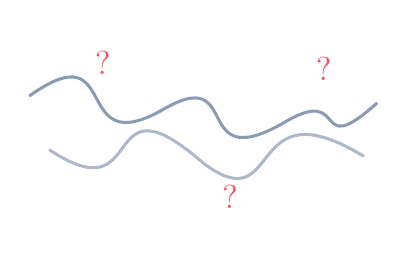
\begin{tikzpicture}[scale=0.85]
  % tangled world
  \draw[FogGray, line width=1.1pt] (0,2.2)
    .. controls (1.4,3.2) and (0.6,1.2) .. (2.0,2.0)
    .. controls (3.2,2.7) and (2.4,1.0) .. (3.8,1.8)
    .. controls (4.8,2.4) and (4.2,1.2) .. (5.2,2.1);
  \draw[FogGray!70, line width=1.1pt] (0.3,1.4)
    .. controls (1.8,0.4) and (1.0,2.6) .. (2.6,1.2)
    .. controls (3.8,0.3) and (3.2,2.4) .. (5.0,1.3);
  \foreach \p in {(1.1,2.7),(3.0,0.7),(4.4,2.6)} \node[text=CoralEmber, font={\DisplayFont\fontsize{12pt}{12pt}\selectfont}] at \p {?};
\end{tikzpicture}
\end{center}
\vspace{2mm}
{\AccentFont\bfseries\lsstyle\textcolor{StormBlue}{THE WORLD BEFORE}}\\[2mm]
\SizeBody{%
\begin{itemize}[leftmargin=4.5mm, itemsep=1.6mm]
  \item An hour of BI setup before the first chart appears
  \item AI flags transactions and can't say \emph{why}
  \item Metrics quoted without their evaluation discipline
  \item Agent “reasoning” that can be quietly rewritten
  \item Compliance teams asked to defend numbers they can't trace
\end{itemize}}
\end{minipage}\hfill
\begin{minipage}[t]{0.06\linewidth}
\vspace{18mm}
\begin{center}
\foreach \y in {0,1.4,2.8,4.2,5.6}{\tikz{\draw[-{Stealth[length=3mm]}, GoldLeaf, line width=1.6pt] (0,0) -- (0.7,0);}\\[6.6mm]}
\end{center}
\end{minipage}\hfill
\begin{minipage}[t]{0.43\linewidth}
\begin{center}
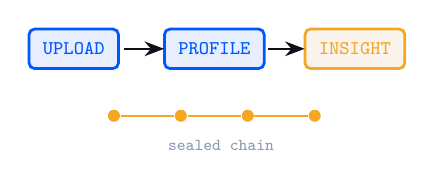
\begin{tikzpicture}[scale=0.85]
  % clean world
  \foreach \x/\t/\c in {0/UPLOAD/ElectricBlue, 2.1/PROFILE/ElectricBlue, 4.2/INSIGHT/GoldLeaf}{
    \node[draw=\c, fill=\c!8!PaperWhite, line width=1pt, rounded corners=2pt, inner sep=5pt,
      font=\ttfamily\bfseries\fontsize{7pt}{7pt}\selectfont, text=\c] at (\x,2.2) {\t};
  }
  \draw[-{Stealth}, CarbonInk, line width=0.9pt] (0.75,2.2) -- (1.35,2.2);
  \draw[-{Stealth}, CarbonInk, line width=0.9pt] (2.9,2.2) -- (3.45,2.2);
  \foreach \x in {0.6,1.6,...,4.4}{\fill[GoldLeaf] (\x,1.2) circle (0.09);}
  \foreach \x in {1.1,2.1,...,3.9}{\draw[GoldLeaf, line width=0.7pt] ({\x-0.4},1.2) -- ({\x+0.4},1.2);}
  \node[text=FogGray, font=\ttfamily\fontsize{6pt}{6.5pt}\selectfont] at (2.2,0.75) {sealed chain};
\end{tikzpicture}
\end{center}
\vspace{2mm}
{\AccentFont\bfseries\lsstyle\textcolor{ElectricBlue}{THE WORLD AFTER}}\\[2mm]
\SizeBody{%
\begin{itemize}[leftmargin=4.5mm, itemsep=1.6mm]
  \item One file drop $\rightarrow$ a BI-grade editable dashboard
  \item Every flag lists the exact signals that drove it
  \item Every metric is held-out and says so on screen
  \item Investigations sealed in a tamper-evident hash chain
  \item “How was this computed?” is a button, everywhere
\end{itemize}}
\end{minipage}

\vspace{7mm}
\begin{minipage}{0.31\linewidth}\masterstat{\StatTests}{tests, green in CI}{ElectricBlue}\end{minipage}\hfill
\begin{minipage}{0.31\linewidth}\masterstat{\StatJawDrop}{flagship features}{GoldLeaf}\end{minipage}\hfill
\begin{minipage}{0.31\linewidth}\masterstat{\StatFabricated}{fabricated metrics}{RegistrarGreen}\end{minipage}

\clearpage

% ════════════════ PAGE 4: THE UNFAIR ADVANTAGE ════════════════
\begin{center}
{\DisplayFont\SizeHeadline{THE UNFAIR ADVANTAGE}}\\[1mm]
{\AccentFont\lsstyle\textcolor{FogGray}{OF NOT BEING A TRADITIONAL ENGINEER}}
\end{center}
\vspace{5mm}

\begin{center}
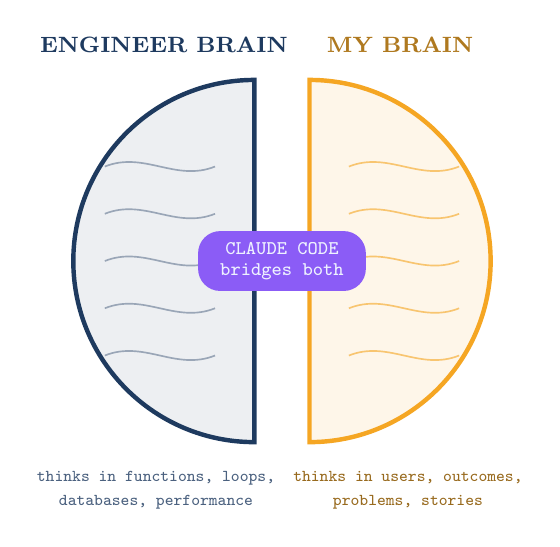
\begin{tikzpicture}
  % split brain: two clean half-discs with a gap between them
  \fill[StormBlue!8]  (-0.35,2.2) ++(90:2.3) arc (90:270:2.3) -- cycle;
  \draw[StormBlue, line width=1.6pt] (-0.35,2.2) ++(90:2.3) arc (90:270:2.3) -- cycle;
  \fill[GoldLeaf!10]  (0.35,2.2) ++(-90:2.3) arc (-90:90:2.3) -- cycle;
  \draw[GoldLeaf, line width=1.6pt] (0.35,2.2) ++(-90:2.3) arc (-90:90:2.3) -- cycle;
  % squiggles (kept inside each half, away from the labels)
  \foreach \y in {1.0,1.6,2.2,2.8,3.4}{
    \draw[StormBlue!45, line width=0.6pt] (-2.25,\y) .. controls (-1.75,{\y+0.2}) and (-1.35,{\y-0.2}) .. (-0.85,\y);
    \draw[GoldLeaf!65, line width=0.6pt] (0.85,\y) .. controls (1.35,{\y+0.2}) and (1.75,{\y-0.2}) .. (2.25,\y);
  }
  % hemisphere titles (above) and thought-styles (below, kept apart)
  \node[text=StormBlue, font={\AccentFont\bfseries\fontsize{8pt}{9pt}\selectfont}] at (-1.5,4.95) {ENGINEER BRAIN};
  \node[text=StormBlue!80, font=\ttfamily\fontsize{6.5pt}{8.6pt}\selectfont, align=center, anchor=north] at (-1.6,-0.35)
    {thinks in functions, loops,\\databases, performance};
  \node[text=GoldLeaf!70!CarbonInk, font={\AccentFont\bfseries\fontsize{8pt}{9pt}\selectfont}] at (1.5,4.95) {MY BRAIN};
  \node[text=GoldLeaf!60!CarbonInk, font=\ttfamily\fontsize{6.5pt}{8.6pt}\selectfont, align=center, anchor=north] at (1.6,-0.35)
    {thinks in users, outcomes,\\problems, stories};
  % the bridge: one violet pill spanning the corpus-callosum gap
  \draw[VioletDream, line width=1.4pt] (-0.85,2.2) -- (0.85,2.2);
  \node[fill=VioletDream, text=IceWhite, rounded corners=8pt, inner xsep=8pt, inner ysep=4pt,
    align=center, font=\ttfamily\bfseries\fontsize{6.8pt}{7.8pt}\selectfont] at (0,2.2)
    {CLAUDE CODE\\bridges both};
\end{tikzpicture}
\end{center}
\vspace{5mm}

\begin{minipage}[t]{0.485\linewidth}
\begin{tcolorbox}[enhanced, colback=GoldLeaf!8!PaperWhite, colframe=GoldLeaf, boxrule=1pt, arc=2mm]
  {\DisplayFont\SizeLead{I ask “why” before “how”}}\\[1.5mm]
  \SizeBody{Verita exists because I interrogated an industry's constraint —
  defensibility — before writing a line of code. The thesis came first; the
  stack served it.}
\end{tcolorbox}
\vspace{2mm}
\begin{tcolorbox}[enhanced, colback=GoldLeaf!8!PaperWhite, colframe=GoldLeaf, boxrule=1pt, arc=2mm]
  {\DisplayFont\SizeLead{I build for users, not reviewers}}\\[1.5mm]
  \SizeBody{The “how was this computed?” button exists because an analyst will
  be \emph{asked}. Features start at the person holding the consequence.}
\end{tcolorbox}
\end{minipage}\hfill
\begin{minipage}[t]{0.485\linewidth}
\begin{tcolorbox}[enhanced, colback=GoldLeaf!8!PaperWhite, colframe=GoldLeaf, boxrule=1pt, arc=2mm]
  {\DisplayFont\SizeLead{I see problems before solutions}}\\[1.5mm]
  \SizeBody{Reading your JD like a crime scene is the skill. The 500 generic AI
  portfolios this season prove how rare “what does this team actually fear?”
  still is.}
\end{tcolorbox}
\vspace{2mm}
\begin{tcolorbox}[enhanced, colback=GoldLeaf!8!PaperWhite, colframe=GoldLeaf, boxrule=1pt, arc=2mm]
  {\DisplayFont\SizeLead{I explain technical things to anyone}}\\[1.5mm]
  \SizeBody{This bundle has a grandmother-grade explanation and an
  engineer-grade one — of the same system, both accurate. That range is the
  JD's “stakeholder communication,” demonstrated.}
\end{tcolorbox}
\end{minipage}

\vspace{6mm}
\masterquote{The argument, made boldly: pair this brain with your engineers and you
don't get a worse engineer — you get a translator who ships. The evidence is the
rest of this bundle.}{the candidate, unhedged}

\clearpage

% ════════════════ PAGE 5: THE JOURNEY ════════════════
\embedgallery{../../04-the-gallery/g9-roadtrip-map.pdf}{g9-roadtrip-map}

% ════════════════ PAGE 6: THE CONSTELLATIONS ════════════════
\embedgallery{../../04-the-gallery/g16-constellation-map.pdf}{g16-constellation-map}

% ════════════════ PAGE 7: WHY THIS COMPANY ════════════════
\begin{center}
{\DisplayFont\SizeHeadline{I DID MY HOMEWORK}}\\[1mm]
{\AccentFont\lsstyle\textcolor{FogGray}{WHY WOLTERS KLUWER, SPECIFICALLY — WITH RECEIPTS}}
\end{center}
\vspace{5mm}

\renewcommand{\arraystretch}{1.7}
\begin{tabularx}{\linewidth}{@{}>{\raggedright\arraybackslash}X >{\raggedright\arraybackslash}X >{\raggedright\arraybackslash}X@{}}
\rowcolor{StormBlue}
{\color{IceWhite}\AccentFont\bfseries YOUR WORLD} & {\color{IceWhite}\AccentFont\bfseries MY UNDERSTANDING} & {\color{IceWhite}\AccentFont\bfseries MY CONTRIBUTION} \\
\SizeBody{WK sells \emph{expert solutions} — software professionals bet their license on, in health, tax, legal, finance.} &
\SizeBody{Your real product is trust under accountability; a wrong answer here has a legal consequence, not a refresh button.} &
\SizeBody{Verita's spine is exactly that value: zero fabricated metrics, every claim traceable. I build like your customers audit.} \\
\SizeBody{FSS/FCC serves compliance teams fighting financial crime under BSA/AML/OFAC regimes.} &
\SizeBody{Analysts drown in alerts; regulators demand that every flag be defensible; explainability is law, not luxury.} &
\SizeBody{A fraud model with honest held-out metrics, an alert queue ranked by evidence, and an NLP analyzer that lists its signals.} \\
\SizeBody{Your JD asks for AI-driven dashboards, forecasting, NLP, GenAI — \emph{plus} stakeholder communication.} &
\SizeBody{The team wants builders whose AI work survives scrutiny and whose explanations survive non-engineers.} &
\SizeBody{Every JD line maps to a shipped feature (the trace document is in the repo) — and this bundle is the communication, performed.} \\
\SizeBody{The industry's next decade: putting agentic AI in front of auditors without losing the trust the brand is built on.} &
\SizeBody{Whoever solves AI \emph{provenance} — what did the machine do and can we prove it — owns that decade.} &
\SizeBody{A working prototype of that answer: the hash-chained, re-runnable Investigator. Small scale, right values, ready to learn yours.} \\
\end{tabularx}

\vspace{7mm}
\begin{tcolorbox}[enhanced, colback=PaleGold, colframe=GoldLeaf, boxrule=1.2pt, arc=2.5mm,
  halign=center, top=4mm, bottom=4mm]
  {\DisplayFont\SizeLead{I didn't build a project that could work for any company.}}\\[1mm]
  {\DisplayFont\SizeLead{I built one that works for yours. There's a difference.}}
\end{tcolorbox}

\clearpage

% ════════════════ PAGE 8: THE NUMBERS ════════════════
\begin{center}
{\DisplayFont\SizeHeadline{WHAT THIS PROJECT ACTUALLY IS,}}\\[1mm]
{\DisplayFont\SizeHeadline{IN NUMBERS}}\\[2mm]
{\AccentFont\lsstyle\textcolor{FogGray}{ALL REAL. REAL BEATS IMPRESSIVE.}}
\end{center}
\vspace{6mm}

\begin{minipage}{0.31\linewidth}\masterstat{\StatTests}{automated tests in CI}{GoldLeaf}\end{minipage}\hfill
\begin{minipage}{0.31\linewidth}\masterstat{\StatTxns}{real transactions}{GoldLeaf}\end{minipage}\hfill
\begin{minipage}{0.31\linewidth}\masterstat{\StatRocAuc}{held-out ROC-AUC}{GoldLeaf}\end{minipage}
\vspace{4mm}

\begin{minipage}{0.31\linewidth}\masterstat{\StatJawDrop}{flagship features}{ElectricBlue}\end{minipage}\hfill
\begin{minipage}{0.31\linewidth}\masterstat{\StatPillars}{product pillars}{ElectricBlue}\end{minipage}\hfill
\begin{minipage}{0.31\linewidth}\masterstat{\StatHypotheses}{SQL tests per investigation}{ElectricBlue}\end{minipage}
\vspace{4mm}

\begin{minipage}{0.31\linewidth}\masterstat{\StatBootSec s}{model warm-boot}{VioletDream}\end{minipage}\hfill
\begin{minipage}{0.31\linewidth}\masterstat{\BuildWeeks}{weeks to shipped}{VioletDream}\end{minipage}\hfill
\begin{minipage}{0.31\linewidth}\masterstat{\StatFabricated}{fabricated metrics}{CoralEmber}\end{minipage}

\vspace{8mm}
\masterinsight{The number that matters most is the last one. Everything else on this
page can be verified \emph{because} of it: drop any CSV into the product and watch the
numbers recompute from your data, live. The demo has no script to fall off.}

\vspace{4mm}
\masterquote{Even where a number is small, it is real — and in the candidate's
industry of choice, a real 0.913 outranks a fabricated 0.99 every day of the audit.}
{the honesty policy, applied to marketing}

\clearpage

% ════════════════ PAGE 9: WHAT HAPPENS NEXT ════════════════
\begin{center}
{\DisplayFont\SizeHeadline{WHAT HAPPENS NEXT}}
\end{center}
\vspace{6mm}

\begin{center}
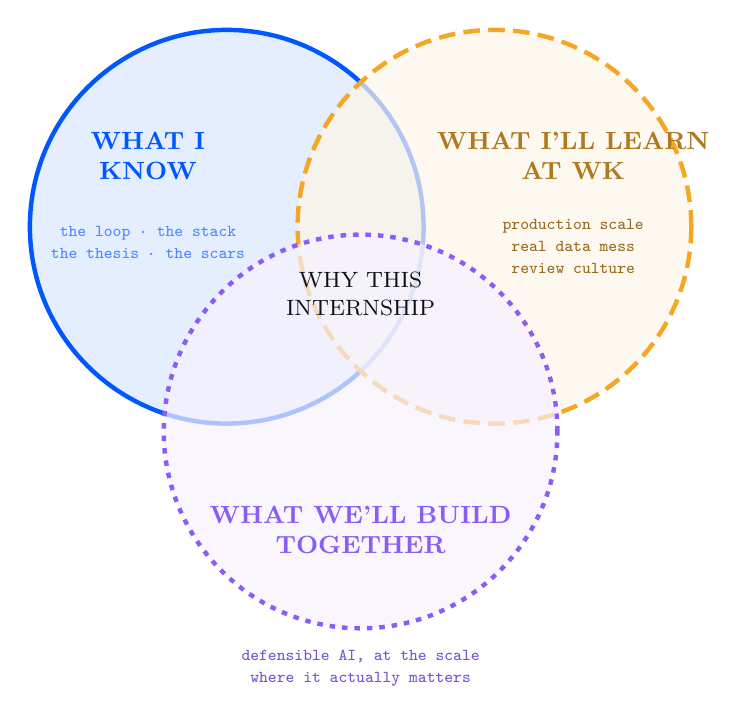
\begin{tikzpicture}
  % three circles venn
  \draw[ElectricBlue, line width=1.6pt, fill=ElectricBlue!10] (-1.7,0) circle (2.5);
  \draw[GoldLeaf, line width=1.6pt, dash pattern=on 6pt off 3pt, fill=GoldLeaf!10, fill opacity=0.7] (1.7,0) circle (2.5);
  \draw[VioletDream, line width=1.6pt, dash pattern=on 2pt off 2.5pt, fill=VioletDream!8, fill opacity=0.7] (0,-2.6) circle (2.5);
  \node[text=ElectricBlue, font={\AccentFont\bfseries\fontsize{9pt}{11pt}\selectfont}, align=center] at (-2.7,0.9)
    {WHAT I\\KNOW};
  \node[text=ElectricBlue!70, font=\ttfamily\fontsize{6.5pt}{8pt}\selectfont, align=center] at (-2.7,-0.2)
    {the loop · the stack\\the thesis · the scars};
  \node[text=GoldLeaf!70!CarbonInk, font={\AccentFont\bfseries\fontsize{9pt}{11pt}\selectfont}, align=center] at (2.7,0.9)
    {WHAT I'LL LEARN\\AT WK};
  \node[text=GoldLeaf!60!CarbonInk, font=\ttfamily\fontsize{6.5pt}{8pt}\selectfont, align=center] at (2.7,-0.25)
    {production scale\\real data mess\\review culture};
  \node[text=VioletDream, font={\AccentFont\bfseries\fontsize{9pt}{11pt}\selectfont}, align=center] at (0,-3.85)
    {WHAT WE'LL BUILD\\TOGETHER};
  \node[text=VioletDream!85!CarbonInk, font=\ttfamily\fontsize{6.5pt}{8pt}\selectfont, align=center, anchor=north] at (0,-5.25)
    {defensible AI, at the scale\\where it actually matters};
  % center
  \node[text=CarbonInk, font={\DisplayFont\fontsize{8.5pt}{10pt}\selectfont}, align=center] at (0,-0.85)
    {WHY THIS\\INTERNSHIP};
\end{tikzpicture}
\end{center}
\vspace{8mm}

\SizeLead{Three specific wants — not “to learn and grow”:}
\vspace{2mm}

\SizeBody{%
\textbf{1.} My first code review from someone who has shipped FCC-grade systems —
I've reviewed my own work as hard as I can alone; the next standard lives here.\\[2mm]
\textbf{2.} Contact with production-scale, genuinely messy institutional data —
the gap between public datasets and reality is the gap between credible and correct.\\[2mm]
\textbf{3.} To watch how senior data scientists defend a model to a stakeholder or
auditor — because that performance is the skill my whole project points toward.}

\clearpage

% ════════════════ PAGE 10: THE CLOSE ════════════════
\thispagestyle{empty}
\begin{tikzpicture}[remember picture, overlay]
  \fill[MidnightNavy] (current page.south west) rectangle (current page.north east);
  \begin{scope}[shift={(current page.south west)}]
    \begin{scope}[opacity=0.5]\stardust{0.3}\end{scope}
  \end{scope}
  \node[text=IceWhite, font={\DisplayFont\fontsize{36pt}{44pt}\selectfont}, align=center]
    at ($(current page.center)+(0,2.6)$) {I DIDN'T COME HERE\\WITH A CV.};
  \node[text=GoldLeaf, font={\DisplayFont\fontsize{36pt}{44pt}\selectfont}, align=center]
    at ($(current page.center)+(0,-1.4)$) {I CAME HERE\\WITH A SOLUTION.};
  \node[text=FogGray, font=\ttfamily\fontsize{9pt}{14pt}\selectfont, align=center]
    at ($(current page.center)+(0,-5.6)$)
    {\MyEmail\ \ ·\ \ \MyGithub\\\MyLinkedin\ \ ·\ \ \MyPhone};
  % QR placeholder
  \draw[IceWhite!50, line width=0.8pt] ($(current page.center)+(-1.05,-8.6)$) rectangle ($(current page.center)+(1.05,-6.5)$);
  \node[text=IceWhite!50, font=\ttfamily\fontsize{6.5pt}{8pt}\selectfont, align=center]
    at ($(current page.center)+(0,-7.55)$) {[QR $\rightarrow$\\GitHub]};
  \node[text=GoldLeaf, font=\ttfamily\fontsize{7pt}{8pt}\selectfont, anchor=south east]
    at ($(current page.south east)+(-0.8,0.8)$)
    {the technical bundle tells the other half of the story.};
\end{tikzpicture}

\end{document}
